\Transcb{yellow}{blue}{The Classical Hamilton and Lagrange formalism}
\begin{itemize}
\item Observation : Nature is lazy
\begin{itemize}
\item Systems evolve performing the least action
\end{itemize}
\item Could we use this feature to derive the laws of nature ?
\begin{itemize}
\item[$\star$] ${\rm d}[action]/{\rm d}[something]=0 \rightarrow$ physical laws ?
\item[$\star$] Need to define {\blue action}
\item[$\star$] Which parameters to describe system and action ?
\item[$\star$] Energy somehow involved $\rightarrow$ description via scalars ?
\end{itemize}
\item Observation : Physicists (and also students !) are lazy
\begin{itemize}
\item Choose the most convenient parameters
\item Choose minimal amount of parameters
\begin{itemize}
\item[$\star$] Free motion $\rightarrow (x,y,z)$
\item[$\star$] Spherical symmetry $\rightarrow (r,\theta,\varphi)$
\item[$\star$] Planar motion $\rightarrow (\rho,\varphi)$ or $(r,\theta)$
\end{itemize}
\end{itemize}
\end{itemize}

\Tr
\begin{itemize}
\item Which and how many parameters to choose ?
\begin{itemize}
\item We can measure {\blue coordinates} and {\blue time}
\item Velocity, acceleration etc... are derived observables\\
      but they describe the evolution of the system
\item Only independent parameters needed
\end{itemize}
\end{itemize}
%
\begin{center}
{\red \shabox{Generalized coordinates}}
\end{center}
%
\begin{itemize}
\item The configuration of a system is uniquely described by any\\
      {\blue complete set} of {\blue independent coordinates} $q_{k}$ ($k=1,\ldots,n$)
\begin{itemize}
\item One is free to choose which coordinates $q_{k}$
\item[] The $q_{k}$ are called {\blue generalized coordinates}
\item Easy to check if the $q_{k}$ are independent
\item But what is the value of $n$ ?
\end{itemize}
\end{itemize}

\Tr
\begin{itemize}
\item Free particle
\begin{itemize}
\item[] $(x,y,z)$ or $(r,\theta,\varphi)$ uniquely determine the position $\rightarrow n=3$
\end{itemize}
\item Particle confined to a plane $(z=0)$
\begin{itemize}
\item[] $(x,y)$, $(r,\theta)$ or $(\rho,\varphi)$ uniquely determine the position $\rightarrow n=2$
\end{itemize}
\item Planar circular motion $(\rho=R=constant)$
\begin{itemize}
\item[] $\varphi$ uniquely determines the position $\rightarrow n=1$
\end{itemize}
\item {\red System of $N$ particles} $\rightarrow n=3N,~2N,~N$ resp. in the above situations
\item[] Definition : {\blue Holonomic constraint}
\begin{itemize}
\item[] {\blue $f(x_{i},y_{j},z_{k},t)=0 ~~~(i,j,k=1,\ldots,N)$}
\end{itemize}
\item[$\ast$] Consider the case of $m$ holonomic constraints (all independent)
\begin{itemize}
\item[] $f_{\alpha}(x_{i},y_{j},z_{k},t)=0 
        ~~~(i,j,k=1,\ldots,N)~(\alpha=1,\ldots,m)$
\end{itemize}
\item[] $\rightarrow$ {\blue $n=(3N-m)$ generalized coordinates needed}
\end{itemize}

\Tr
\begin{itemize}
\item[$\star$] Previous example of planar circular motion
\begin{itemize}
\item Only 1 particle $\rightarrow N=1$
\item Constraints : $z=0$ and $x^{2}+y^{2}-R^{2}=0 \rightarrow m=2$
\item[] $\Rightarrow n=3-2=1$ generalized coordinates needed
\item We had chosen $\varphi$ for this case
\end{itemize}
\item[$\star$] Add a second particle in the same plane at radius $R_{2}$
\item[] Use cylindrical coordinates $(\rho,\varphi)$ for simplicity
\begin{itemize}
\item Now we have 2 particles $\rightarrow N=2$
\item Constraints :    $z_{1}=0$ ~~~$\rho_{1}-R=0$
\item[] \hspace{43mm}  $z_{2}=0$ ~~~$\rho_{2}-R_{2}=0$
\item[] $\rightarrow m=4$
\item[] $\Rightarrow n=6-4=2$ generalized coordinates needed
\item Obviously we can choose $\varphi_{1}$ and $\varphi_{2}$
\end{itemize}
\end{itemize}

\Tr
\begin{itemize}
\item[$\star$] Assume both particles have fixed relative position
\item[] $\rightarrow$ fixed angle $\alpha$ between them
\begin{itemize}
\item We still have 2 particles $\rightarrow N=2$
\item Constraints :    $z_{1}=0$ ~~~$\rho_{1}-R=0$
\item[] \hspace{43mm}   $z_{2}=0$ ~~~$\rho_{2}-R_{2}=0$
\item[] \hspace{43mm}   $\varphi_{1}-\varphi_{2}-\alpha=0$
\item[] $\rightarrow m=5$
\item[] $\Rightarrow n=6-5=1$ generalized coordinates needed
\item We can choose $\varphi_{1}$ in this case
\end{itemize}
\item Note :
\begin{itemize}
\item[] {\blue $n$} is called the {\blue number of degrees of freedom} of the
        system
\end{itemize}
\end{itemize}

\Tr
\begin{center}
{\red \shabox{Hamilton's variational principle}}
\end{center}
%
\begin{itemize}
\item Systems evolve along a certain path in space-time
\item Relate the {\blue action} to the {\blue path-integral} ${\cal P}={\displaystyle \int_{t_{1}}^{t_{2}}} L \,{\rm d}t$
\item[] with : $L \equiv$ some function related to the system's energy ($L \sim E_{kin}$ and $E_{pot}$)
\begin{itemize}
\item[$\star$] Use generalized coordinates for convenience $\rightarrow L=L(q,\dot{q},t)$ 
\end{itemize}
\item {\blue ${\cal P}$ is an extremum along the actual path}
\begin{itemize}
\item[] Actual path $\rightarrow \delta{\cal P}=
  \delta{\displaystyle \int_{t_{1}}^{t_{2}}} L(q,\dot{q},t) \,{\rm d}t=
  {\displaystyle \int_{t_{1}}^{t_{2}}} \delta L(q,\dot{q},t) \,{\rm d}t=0$
\end{itemize}
\item[] with : $\delta \equiv$ infinitessimal variation of any system parameter\\
 \hspace*{35mm} away from the actual path value
\item Note : The endpoints at $t_{1}$ and $t_{2}$ have to remain fixed
             on the actual path
\end{itemize}
\begin{itemize}
\item[$\star$] Regard $\delta {\cal P}$ as an investigation of the
               value of ${\cal P}$
\begin{itemize}
\item Like estimating the weight of an object by trying to lift it
\end{itemize}
\end{itemize}

\Tr
\begin{itemize}
\item Consider conservative systems with time-independent holonomic constraints
\begin{itemize}
\item No explicit time dependence of $L \rightarrow L=L(q,\dot{q})$
\end{itemize}
\item As usual we can now write :
\begin{itemize}
\item[] {\blue ${\displaystyle \int_{t_{1}}^{t_{2}}} \delta L \,{\rm d}t=
 {\displaystyle \int_{t_{1}}^{t_{2}} \sum_{k=1}^{n}
 \left( \frac{\partial L}{\partial q_{k}} \delta q_{k}
 + \frac{\partial L}{\partial \dot{q}_{k}} \delta\dot{q}_{k} \right)}
 {\rm d}t \equiv 0$} ~~~(1)
\end{itemize}
\item[$\star$] Note that : ${\blue \delta\dot{q}_{k}=\frac{{\rm d}}{{\rm d}t}(\delta q_{k})}$ ~~~(2)
\item[]  Since : $\delta \dot{q}=\delta {\displaystyle 
 \lim_{\Delta t \rightarrow 0} \frac{q(t+\Delta t)-q(t)}{\Delta t}=
 \lim_{\Delta t \rightarrow 0} \frac{\delta q(t+\Delta t)- \delta q(t)}{\Delta t}=
 \frac{{\rm d}}{{\rm d}t}(\delta q)}$
\item (1)\&(2) yields~:
 ${\displaystyle \int_{t_{1}}^{t_{2}} \sum_{k=1}^{n}
 \left( \frac{\partial L}{\partial q_{k}} \delta q_{k}
 + \frac{\partial L}{\partial \dot{q}_{k}}
 \frac{{\rm d}}{{\rm d}t}(\delta q_{k}) \right)} {\rm d}t=0$
\item Integration by parts of the second term yields :
\item[]
$\displaystyle \left[ \sum_{k=1}^{n}
 \frac{\partial L}{\partial\dot{q}_{k}}\delta q_{k} \right]_{t_{1}}^{t_{2}}
 - \int_{t_{1}}^{t_{2}} \sum_{k=1}^{n} \frac{{\rm d}}{{\rm d}t}
 \left( \frac{\partial L}{\partial\dot{q}_{k}} \right) \delta q_{k}\,{\rm d}t$
\item[$\star$] Note : 
$\displaystyle \left[ \sum_{k=1}^{n}
 \frac{\partial L}{\partial\dot{q}_{k}}\delta q_{k} \right]_{t_{1}}^{t_{2}}=0$
~~~(fixed endpoints)
\item This finally yields :
$\displaystyle \int_{t_{1}}^{t_{2}} \sum_{k=1}^{n}
 \left[ \frac{\partial L}{\partial q_{k}}
 - \frac{{\rm d}}{{\rm d}t}
 \left( \frac{\partial L}{\partial\dot{q}_{k}} \right) \right]
 \delta q_{k}\,{\rm d}t=0$
\item[$\star$] Should hold for all independent $q_{k}$ and $\delta q_{k}$
\item[] In other words :
\end{itemize}
%
\begin{center}
 {\red \shabox{$\displaystyle \frac{\partial L}{\partial q_{k}}
 - \frac{{\rm d}}{{\rm d}t}
 \left( \frac{\partial L}{\partial\dot{q}_{k}} \right)=0$}}
\end{center}
%
\begin{itemize}
\item[] These equations are called the {\blue Lagrangian equations of\\
        motion} and $L$ is called the {\blue Lagrangian} of the system
\end{itemize}

\Tr
\begin{itemize}
\item But what is the expression for $L(q,\dot{q})$ ?
\begin{itemize}
\item The Lagrange equations should yield Newton's laws
\item Guesswork, try and error by Lagrange $(\sim 1800)$
\end{itemize}
\end{itemize}
%
\begin{center}
{\red \fbox{$L=T-V$}}
\end{center}
%
\begin{itemize}
\item[$\star$] No deep reason behind expression for $L$, it just works !
\item[] Note :
\begin{itemize}
\item Lagrange equations only involve scalars $\rightarrow$ easy
\item Lagrange equations only valid for conservative systems
\end{itemize}
\end{itemize}

\Tr
\begin{center}
{\red \shabox{Recipe for Lagrangian analysis}}
\end{center}
%
\begin{enumerate}
\item Determine the number of degrees of freedom $(n)$ of the system
\item Select a suitable set of generalized coordinates $q_{k}$
\item Find relation between Cartesian- and generalized coordinates
\item Express $T$ and $V$ in terms of Cartesian coordinates
\item Express $T$ and $V$ in terms of generalized coordinates
\item Write $L$ in terms of generalized coordinates
\item Apply the Lagrange equations
\item Solve the diff. equations $\rightarrow$ Problem solved !
\end{enumerate}
%
\begin{itemize}
\item[$\star$] Steps (3) and (4) may be skipped in obvious situations
\end{itemize}

\Tr
\begin{itemize}
\item Example : Free particle
\begin{enumerate}
\item Only 1 particle $(N=1)$, no constraints $(m=0)$ $\rightarrow n=3$
\item Just choose the Cartesian $(x,y,z)$
\item Trivial
\item $T=\frac{1}{2}m(\dot{x}^{2}+\dot{y}^{2}+\dot{z}^{2})$ and $V=0$
\item Same as above
\item $L=\frac{1}{2}m(\dot{x}^{2}+\dot{y}^{2}+\dot{z}^{2})$
\item Lagrange equations :
 {\blue $\displaystyle
 \frac{{\rm d}}{{\rm d}t} \left( \frac{\partial L}{\partial\dot{q}_{k}} \right)=
 \frac{\partial L}{\partial q_{k}}$}
\begin{itemize}
\item[$\star$] $\frac{\rm d}{{\rm d}t}(m\dot{x})=0 \rightarrow \ddot{x}=0$
\item[$\star$] $\frac{\rm d}{{\rm d}t}(m\dot{y})=0 \rightarrow \ddot{y}=0$
\item[$\star$] $\frac{\rm d}{{\rm d}t}(m\dot{z})=0 \rightarrow \ddot{z}=0$
\end{itemize}
\item Usual procedure $\rightarrow$ Newtonian results !
\end{enumerate}
\end{itemize}
%
\begin{itemize}
\item[$\star$] Note : Lagrange equations yield $m\dot{x}=p_{x}=constant$ etc.
\item[] Obviously due to the fact that $L$ independent of $q_{k}$
\end{itemize}
%
\begin{center}
{\red \shabox{Generalized momenta}}
\end{center}
%
\begin{itemize}
\item[] Define : {\blue \fbox{$\displaystyle  p_{k} \equiv \frac{\partial L}{\partial\dot{q}_{k}}$}}
 $\rightarrow$ Lagrange equations : $\displaystyle  \dot{p}_{k}=\frac{\partial L}{\partial q_{k}}$
\item Fundamental physics law :
\end{itemize}
%
\begin{center}
{\red \shabox{Translational invariance $\rightarrow$ Momentum conservation}}
\end{center}
%
\begin{itemize}
\item From Quantum Mechanics or Special Relativity we have seen that also :
\end{itemize}
%
\begin{center}
{\red \shabox{Time invariance $\rightarrow$ Energy conservation}}
\end{center}
%
\begin{itemize}
\item[$\ast$] Reflects the Noether theorem : {\blue Some invariance $\Leftrightarrow$ Some Conservation}
\end{itemize}

\Tr
\begin{itemize}
\item Example : Particle in central force field
\begin{enumerate}
\item Planar motion $(z=0) \rightarrow n=2$
\item Choose plane polar coordinates $(r,\theta)$
\item Coordinate relations :
\begin{itemize}
\item[] $x=r\cos(\theta)$ ~~~
        $\dot{x}=\dot{r}\cos(\theta)-r\dot{\theta}\sin(\theta)$
\item[] $y=r\sin(\theta)$ ~~~
        $\dot{y}=\dot{r}\sin(\theta)+r\dot{\theta}\cos(\theta)$
\end{itemize}
\item $T=\frac{1}{2}m(\dot{x}^{2}+\dot{y}^{2})$ ~~~ $V=V(\sqrt{x^{2}+y^{2}}\,)$
\item $T=\frac{1}{2}m(\dot{r}^{2}+r^{2}\dot{\theta}^{2})$ ~~~ $V=V(r)$
\item $L=\frac{1}{2}m(\dot{r}^{2}+r^{2}\dot{\theta}^{2})-V(r)$
\item Lagrange equations :
\begin{itemize}
\item[$\star$] $mr\dot{\theta}^{2}-\frac{\partial V}{\partial r}-m\ddot{r}=0$
               $\rightarrow m\ddot{r}=mr\dot{\theta}^{2}+f(r)$
\item[$\star$] $\frac{\rm d}{{\rm d}t}(mr^{2}\dot{\theta})=0$
               $\rightarrow |\vec{L}|=constant$
\end{itemize}
\item Identical to Kepler orbit situation $\rightarrow$ Same results !
\end{enumerate}
\end{itemize}

\Tr
\begin{center}
{\red \shabox{Hamilton's equations of motion}}
\end{center}
%
\begin{itemize}
\item Define the {\red Hamiltonian} :
 {\red \fbox{$H \equiv {\displaystyle \sum_{k=1}^{n}} \dot{q}_{k}p_{k}-L$}}
\item[] $\rightarrow \delta H = {\displaystyle \sum_{k=1}^{n}
 \left[ p_{k}\delta\dot{q}_{k}+\dot{q}_{k}\delta p_{k}-
 \frac{\partial L}{\partial\dot{q}_{k}}\delta\dot{q}_{k}-
 \frac{\partial L}{\partial q_{k}}\delta q_{k} \right]}$
\item[$\star$] Using :
 $\displaystyle p_{k}=\frac{\partial L}{\partial \dot{q}_{k}}$ and
 $\displaystyle \dot{p}_{k}=\frac{\partial L}{\partial q_{k}}
 \rightarrow {\blue \delta H={\displaystyle \sum_{k=1}^{n}}
                    [\dot{q}_{k}\delta p_{k}-\dot{p}_{k}\delta q_{k}]}$ ~~~(1)
\item[$\star$] So : $H=H(p_{k},q_{k})
 \rightarrow {\blue \delta H={\displaystyle \sum_{k=1}^{n}
 \left[ \frac{\partial H}{\partial p_{k}}\delta p_{k}+
 \frac{\partial H}{\partial q_{k}}\delta q_{k} \right]}}$ ~~~(2)
\item (1) \& (2) directly yield :
{\red \shabox{$\displaystyle
 \frac{\partial H}{\partial p_{k}}=\dot{q}_{k}$ ~~and~~
 $\displaystyle \frac{\partial H}{\partial q_{k}}=-\dot{p}_{k}$}}
\end{itemize}

\Tr
\begin{itemize}
\item Hamilton's equations hold for more general systems\\
 (non-conservative, explicit time dependence of $L$, ...)
\item Simple conservative systems $\rightarrow H=T+V$
\end{itemize}
%
\begin{center}
{\blue And still something is wrong !}\\[1cm]
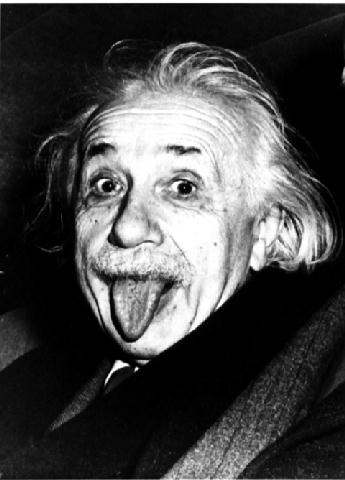
\includegraphics[keepaspectratio,height=10cm]{einstein}
\end{center}